\documentclass[isoft]{poster_class_UofC}

\usepackage{lipsum}
\usepackage{natbib}
\usepackage{booktabs}
\usepackage{subfig} 
\usepackage{amsmath} 
\usepackage{textcomp} 
\usepackage{url}  
\usepackage{hyperref}
\usepackage[utf8]{inputenc}
\usepackage[english]{babel}

%%%%%%%%%%%%%%%%%%%%%%%%%%%%%%%%%%%%%%%%%
%%               Configs               %%
%%%%%%%%%%%%%%%%%%%%%%%%%%%%%%%%%%%%%%%%%

% Choose one of the section color {ufglhblue | ufgdkblue | dkblue | black | gold}
\setsectioncolor{red} 
\setsubsectioncolor{gold}

% Define width of the rule or hide it by setting 0pt or commenting the command 
%\setcolumnseprule{2pt}

% Inform the paths to the logo files or leave empty one or both parameters. 
% There are three options [ T | M | B ] to positioning them.
%\setlogos[T]{images/uc-vert-rgb}

% Choose one of the background options {1 | 2 | 3}. 
% Actually, one can select any graphic file in backgrounds directory. 
\setbackground{1}

% Resize the title to keep it in two lines 
\settitlesize{64pt}{60pt}

% General info
\title{\uppercase{U-Net image segmentation does not improve multi-level \\regression model performance when predicting cell counts \\from fluorescene microscopy images }} 

\author{Andrew Pohl\textsuperscript{1}, Dylan Loader\textsuperscript{2}, Mingkuan ...\textsuperscript{2}} 

\department{\textsuperscript{1}Faculty of Kinesiology. \textsuperscript{2}Department of Mathematics and Statistics \\ 
University of Calgary}

\email{ \text{andrew.pohl@ucalgary.ca, dylan.loader@ucalgary.ca, mingkuan@ucalgary.ca} }

%\class{Projeto Ciência no Parque}

\posteryear{2019}

\copyrightholder{Department of Mathematics and Statistics - University of Calgary}

%%%%%%%%%%%%%%%%%%%%%%%%%%%%%%%%%%%%%%%%%
%%           End configs               %%
%%%%%%%%%%%%%%%%%%%%%%%%%%%%%%%%%%%%%%%%%

\pagestyle{fancy}
\begin{document}
    \begin{poster}
    
    %%%%%%%%%%%%%%%%%%%%%%%%%%%%%%%%%%%%%%%%%
    %%             Begin poster            %%
    %%%%%%%%%%%%%%%%%%%%%%%%%%%%%%%%%%%%%%%%%
    \section{Introduction}
    
        \lipsum[3-5]
        
    \section{Methods}%
        
        \subsection{Data Preparation}
       To develop a robust training and testing environment which allowed for testing of model performance the supplied training data was split randomly into a training set ($80\%$) and validation set ($20\%$).  Parameters for regression models were estimated from the ....images in the training set and then performance assessed on the .... images within the with-held validation set.  Images were used in the supplied .TIF format with no further image processing performed. Thus images contained between 1 and 100 cells identified by one of two cell staining techniques and subjected to one of three levels of bluing.
        \subsection{U-Net Training}
The U-Net [CITATION] is a common encoder-decoder neural network architecture which has been shown to be effective in image segmentation tasks [CITATION]. The U-Net we used to segment cells from the background of the supplied images was simplified from that used by [CITE NATURE PAPER].  It consisted of 5 layered encoder consisting of 2-dimensional convolution layers of 32,64,128,256 and 512 filters with 3x3 kernals activated by leaky rectified linear units (ReLU) Max pooling was performed between each layer, effectively halving the resolution of each feature map.  Following the encoder an equivalent 5 layer decoder network (similar but reversed layers as the encoder) was constructed with characteristic up-convolution performed immediately prior to each convolution layer.  Finally a 1 dimensional convolution layer with 1x1 kernal activated with the soft-max function was used to produce the segmentation mask for each image. The architecture for the U-Net is outline in figure \ref{fig:U-NET}.
        
        \begin{figure}
                    \centering
            \captionsetup{type=figure}
            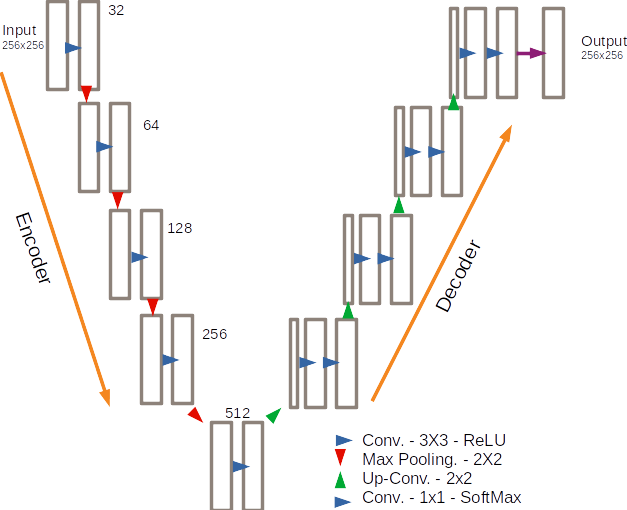
\includegraphics[scale=1]{./images/UNet_Arch.png}
            \caption{U-Net architecture used for image segmentation.}
            \label{fig:U-NET}
        \end{figure}
        
        To train the U-Net 830 images with ground-truth segmentation masks were obtained from [CITE BBBC].  NNet training was performed in Python v. 3... with the Keras interface to tensorflow \cite{chollet2015keras}.  To increase the training set size (and improve image segmentation performance) a data-generator was constructed which rescaled images to 256x256 pixels and performed random rotations along with horizontal and vertical image shifts.  The network was trained using the ADAM optimiser with a learning rate of 0.0001 and dice coefficient loss as the loss function.  Training was performed using a .... CPU on a Lenovo thinkpad P51 laptop.  Training was completed for 7 epochs with a batch size of 64 based on a early stopping condition when no improvement in was observed on a random 5\% validation set.  Once trained the U-Net was used to produce segmentation masks for the ... images in the respective train and validation sets used for subsequent regression analysis.  Examples of segmentation performance are shown for 3 training images in figure \ref{fig:segmentation_performance}.
        
           \begin{figure}
            \centering
            \captionsetup{type=figure}
            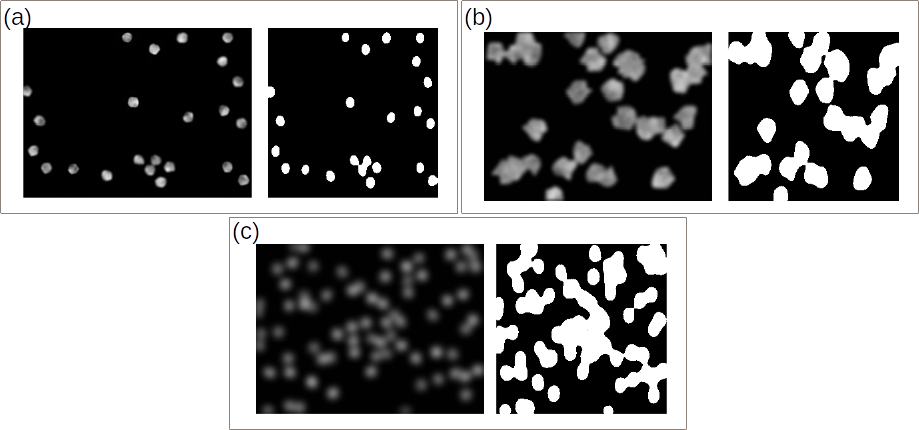
\includegraphics[scale=1.5]{./images/cell_images.png}
            \caption{Performance of Unet image segmentation for low (a), medium (b), and high (c) blur images with nulceli (a, c) and cytoplasm (b) stains.  Segmentation images are on the right with original images on the left of each block.}
            \label{fig:segmentation_performance}
        \end{figure}     
          
        \subsection{Regression Models}      
     A Bayesian implementation of polynomial regression was applied to predict the number of cells from either a raw image or U-Net generated image mask.  The sum of the normalised pixels for each image $x_i$ was used as the sole covariate to estimate cell count for each image ($y_i$).   For the U-Net generated image masks each pixel was either 0 or 1 dependent on whether the pixel was identified as a cell or not, for the raw images pixels were in the range $[0,255]$ but were subsequently normalised by dividing the observed pixel intensity by $255$ to provide pixels within the range $[0,1]$.  
     Three polynomial regression models were examined: (i) a single level model where parameter values were estimated from all images, (ii) a random slopes model where slope regression parameters ($\beta_1, \beta_2$) were allowed to vary for each stain/blur level group $j = 1, ..., 6$ and (iii) a model where both slopes ($\beta_1, \beta_2$) and intercepts ($\beta_0$) were allowed to vary for each group.  The full varying slope and intercept model is outlined in  (\ref{eqn:RegressionModel}).
\begin{align}
y_{ij} \sim N(\mu_{ij}, \sigma^2) \nonumber\\
\mu_{ij} = {\beta_0}_{ij} + {\beta_1}_{ij} x_{ij} + {\beta_2}_{ij} x_{ij}^2 \label{eqn:RegressionModel}
\end{align}     
     Parameters of each model were estimated via Markov Chain Monte Carlo implemented in JAGS [CITE JAGS]. Weakly informative priors were utilised for each parameter. Four chains of 10000 iterations were used with convergence examined via visual examination of traceplots and determination of the R-hat and effective sample size statistics [Cite GELMAN].     
        
        \section{Results}%
The RMSE of predicting the number of cells from images within the validation is outlined \ref{tab:Results}.  RMSE reduces with each layer of complexity with the most complex model examined producing the most accurate predictions.  While RMSE is similar between raw images and image segmentation masks it is notable that performance is consistently better when raw images were used.  

There was considerable evidence to suggest differences in parameter estimates between when raw images were used vs when U-Net generated segmentation masks were used.  While this is partially explained by differing numbers of pixels between the two images sources, U-Net segmentation had the effect of making differences between the 3 levels of blurring and two different stains become more aparent.  This is outlined in figure \ref{fig:Results} which compares the varying slopes and intercepts model between raw image and U-Net masks. This improved ability to separate the varying blur groups when U-Net masks were applied may be attributed to ......
        
                \vspace{1cm}
            \begin{table}
                \centering
                \captionsetup{type=table}
                \caption{\textit{Corpus} utilizados no estudo}
                \label{Corpus}
                \renewcommand{\arraystretch}{1.2}
                \resizebox{0.47\textwidth}{!}{%
                \begin{tabular}{lcccclcl}
                    \hline
                    &\textbf{Corpus}    &  \textbf{Caracteres únicos} &    &  \textbf{Total de linhas}  &  & \textbf{Total de caracteres} &  \\ \hline
                    &SBSEThesis         & 88  &    &    2.311     &        & 771.179 &  \\ 
                    &Bible              & 63  &    &    32.359   &        & 3.924.374 &  \\
                    &JavaCode           & 69  &    &    436.565  &        & 12.053.424 &  \\ \hline
                \end{tabular}
            }
            \end{table}
            \vspace{1cm}
            
            
            
    
        \section{Conclusions}
    
            \lipsum[15]
        \section{Future Directions}

    
        \section{Acknowledgements}

        \bibliographystyle{abbrv}
        \bibliography{refs}
    
    %%%%%%%%%%%%%%%%%%%%%%%%%%%%%%%%%%%%%%%%%
    %%               End poster            %%
    %%%%%%%%%%%%%%%%%%%%%%%%%%%%%%%%%%%%%%%%%
    
    \end{poster}

\end{document}

 
